\subsection{Evaluation}
\label{subsec:revpar_eval}
Nachdem im vorherigen Abschnitt die Vorhersage normierter RevPAR-Werte mittels eines definierten Code-Abschnitts erfolgte, rückt nun die Frage nach der Genauigkeit dieser Vorhersagen in den Vordergrund. Diese Sektion widmet sich daher einer eingehenden Untersuchung der Wirksamkeit der vorhergesagten Werte für das Jahr 2023. Ziel dieser Evaluation ist es, die Übereinstimmung der prognostizierten Werte mit den tatsächlichen Daten zu bewerten und die Zuverlässigkeit des Modells bei der Vorhersage zu prüfen.
\newline
\newline
Um dieses Ziel zu erreichen, werden verschiedene Metriken wie der R2-Score, der Root-Mean-Square-Error und der Mean-Absolute-Error verwendet, um die Abweichungen zwischen den Vorhersagen und den realen Werten zu quantifizieren. Darüber hinaus erfolgt ein direkter Vergleich zwischen dem entwickelten Modell und dem aktuellen Live-Modell, das derzeit von Kunden verwendet wird. Diese Gegenüberstellung ermöglicht es, fundierte Entscheidungen über das weitere Vorgehen zu treffen, basierend auf einem direkten Vergleich der Leistungsfähigkeit beider Modelle.

\begin{figure}[h]
    \centering
    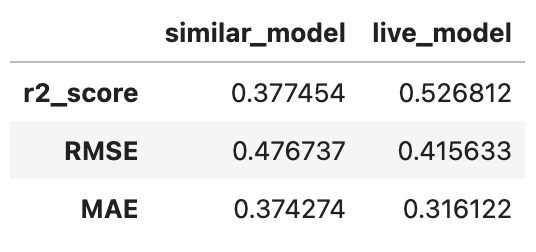
\includegraphics[width=1\textwidth, center]{revpar_eval_1.png}
    \caption[Evaluation der beiden Modelle für das erste Benchmark-Hotel]{Evaluation der beiden Modelle für das erste Benchmark-Hotel}
    \label{img:revpar_eval_1}
\end{figure}

Die Darstellung in Abbildung \ref{img:revpar_eval_1} präsentiert die Ergebnisse der einzelnen Modelle und ermöglicht gleichzeitig einen direkten Vergleich zwischen ihnen. Dabei fällt auf, dass das aktuell verwendete Live-Modell im Vergleich zum Similar-Modell eine bessere Leistung für dieses spezifische Hotel aufweist. Es ist jedoch wichtig zu beachten, dass das Similar-Modell gänzlich auf hotel-spezifische Daten verzichtet und trotzdem nur eine geringfügige Differenz aufweist.
\newline
\newline
Die Berücksichtigung eines einzelnen Hotels allein für diese Evaluation könnte als begrenzt angesehen werden. Daher wird die Analyse um das zweite Benchmark-Hotel erweitert, um festzustellen, wie die einzelnen Modelle dort abschneiden. Dies ermöglicht eine umfassendere Beurteilung der Leistungsfähigkeit der Modelle über verschiedene Kontexte hinweg.

\begin{figure}[h]
    \centering
    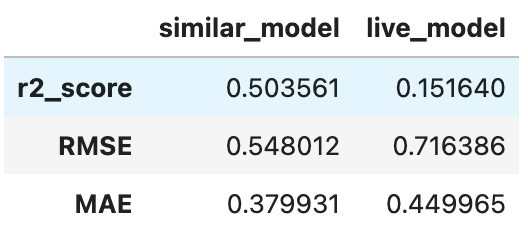
\includegraphics[width=1\textwidth, center]{revpar_eval_2.png}
    \caption[Evaluation der beiden Modelle für das zweiten Benchmark-Hotel]{Evaluation der beiden Modelle für das zweiten Benchmark-Hotel}
    \label{img:revpar_eval_2}
\end{figure}

Die Einbeziehung der Ergebnisse des zweiten Benchmark-Hotels, wie sie in Abbildung \ref{img:revpar_eval_2} dargestellt sind, verdeutlicht signifikante Unterschiede in der Leistung des Live-Modells. In diesem Szenario erweist sich das Similar-Modell als deutlich überlegen, obwohl es ohne hotel-spezifische Daten arbeitet. Diese Erkenntnis unterstreicht, dass die Modelle je nach individuellen Hotelkontexten unterschiedlich gut abschneiden können.

\subsection{Zwischenfazit}
\label{subsec:revpar_fazit}
Die präsentierten Ergebnisse in Abschnitt \emph{\nameref{subsec:revpar_eval}} legen nahe, dass das Similar-Modell trotz des Fehlens hotel-spezifischer Daten ein valide Ansatz zur Vorhersage normierter RevPAR-Werte darstellt. Basierend auf diesen Erkenntnissen wurde beschlossen, diesen Ansatz für die dynamische Preisgenerierung von Hotels ohne Verfügbarkeit von Vergangenheitsdaten zu nutzen.

